\documentclass[10pt,a4paper]{article}
\usepackage[paper=a4paper, left=1.5cm, right=1.5cm, bottom=2.0cm, top=1.6cm]{geometry}
\usepackage[utf8]{inputenc} % para poder usar tildes en archivos UTF-8
\usepackage[spanish]{babel} % para que comandos como \today den el resultado en castellano
\usepackage[conEntregas]{caratula}
\usepackage{amsmath}
\usepackage[colorlinks=true, linkcolor=blue]{hyperref}
\usepackage[section]{placeins}

\usepackage{ifpdf}
\usepackage{multicol}
\usepackage{caption}
\usepackage{subcaption}
\usepackage{listings}

\begin{document}

\titulo{Trabajo Pr\'actico 1}
\subtitulo{Wiretapping}

\fecha{\today}

\materia{Teoría de las comunicaciones}

%\grupo{Grupo ?}

\integrante{Barbeito, Nicol\'as}{147/10}{barbeiton@yahoo.com.ar}
\integrante{Interlandi, Daniel}{773/00}{danielinterlandi@gmail.com}
\integrante{Ladelfa, Hern\'an Nahuel}{318/04}{nahueladelfa@gmail.com}

\maketitle
\tableofcontents
\newpage
  
\section{Resúmen}

El objetivo de este trabajo es el de experimentar con las herramientas provistas por el protocolo ICMP para analizar las rutas tomadas por los paquetes hasta alcanzar su destino. Además se analizará la existencia de saltos entre nodos intercontinentales en las rutas de los experimentos.

\section{Introducción}

\newpage
\section{Primera consigna: capturando tráfico}

\subsection{Herramienta}

Para realizar las capturas de las redes, se desarrollo un script en el lenguaje Python integrado con la herramienta Scapy.
Este script escucha pasivamente la red capturando los paquetes que son almacenados en distintos archivos para su posterior análisis.

En los archivos se guarda la información, probabilidad y entropía de las 2 fuentes elegidas. Por tipo de protocolo para los paquetes Ethernet y por IP para la captura de paquetes ARP.

Un 3 archivo de formato json, contiene la información de manera organizada para poder ser leído por otro script desarrollado utilizado para generar distintos gráficos.

Este segundo script genera gráficos como histogramas, de torta y grafos según paquetes ARP enviados.

\subsection{Ejecución}

Para la ejecución de la herramienta, debemos ejecutar los siguiente comandos desde una terminal en el sistema operativo Linux.

\begin{lstlisting}[language=bash]
  $ sudo ./sniffer.py <outputfile> <timeout> 
\end{lstlisting}

Para la ejecución del graficador:

\begin{lstlisting}[language=bash]
  $ sudo ./plot.py <outputfile> 
\end{lstlisting}

\newpage
\section{Resultados}

\subsection{Segunda Consigna: Gráficos y Análisis}

\subsubsection{Red Doméstica}

Para la primera captura, se eligió una red domestica de uno de los integrantes del grupo. Los dispositivos conectados a la red en este caso fueron, 3 computadoras, 2 celulares, un televisor SmartTV y un Apple TV. Todos estos conectados al modem del proveedor de internet.
La captura duró aproximadamente 30 minutos.
Al ser una red pequeña podemos distinguir fácilmente los nodos destacados.
La Figura~\ref{fig:red_domestica_network}. muestra 2 nodos destacados. 192.168.0.1 que corresponde al router  y el nodo 192.168.0.27 correspondiente al SmartTV que en el momento de la captura de los paquetes, el mismo se encontraba actualizandose.

\begin{figure}[h!]
  \centering
   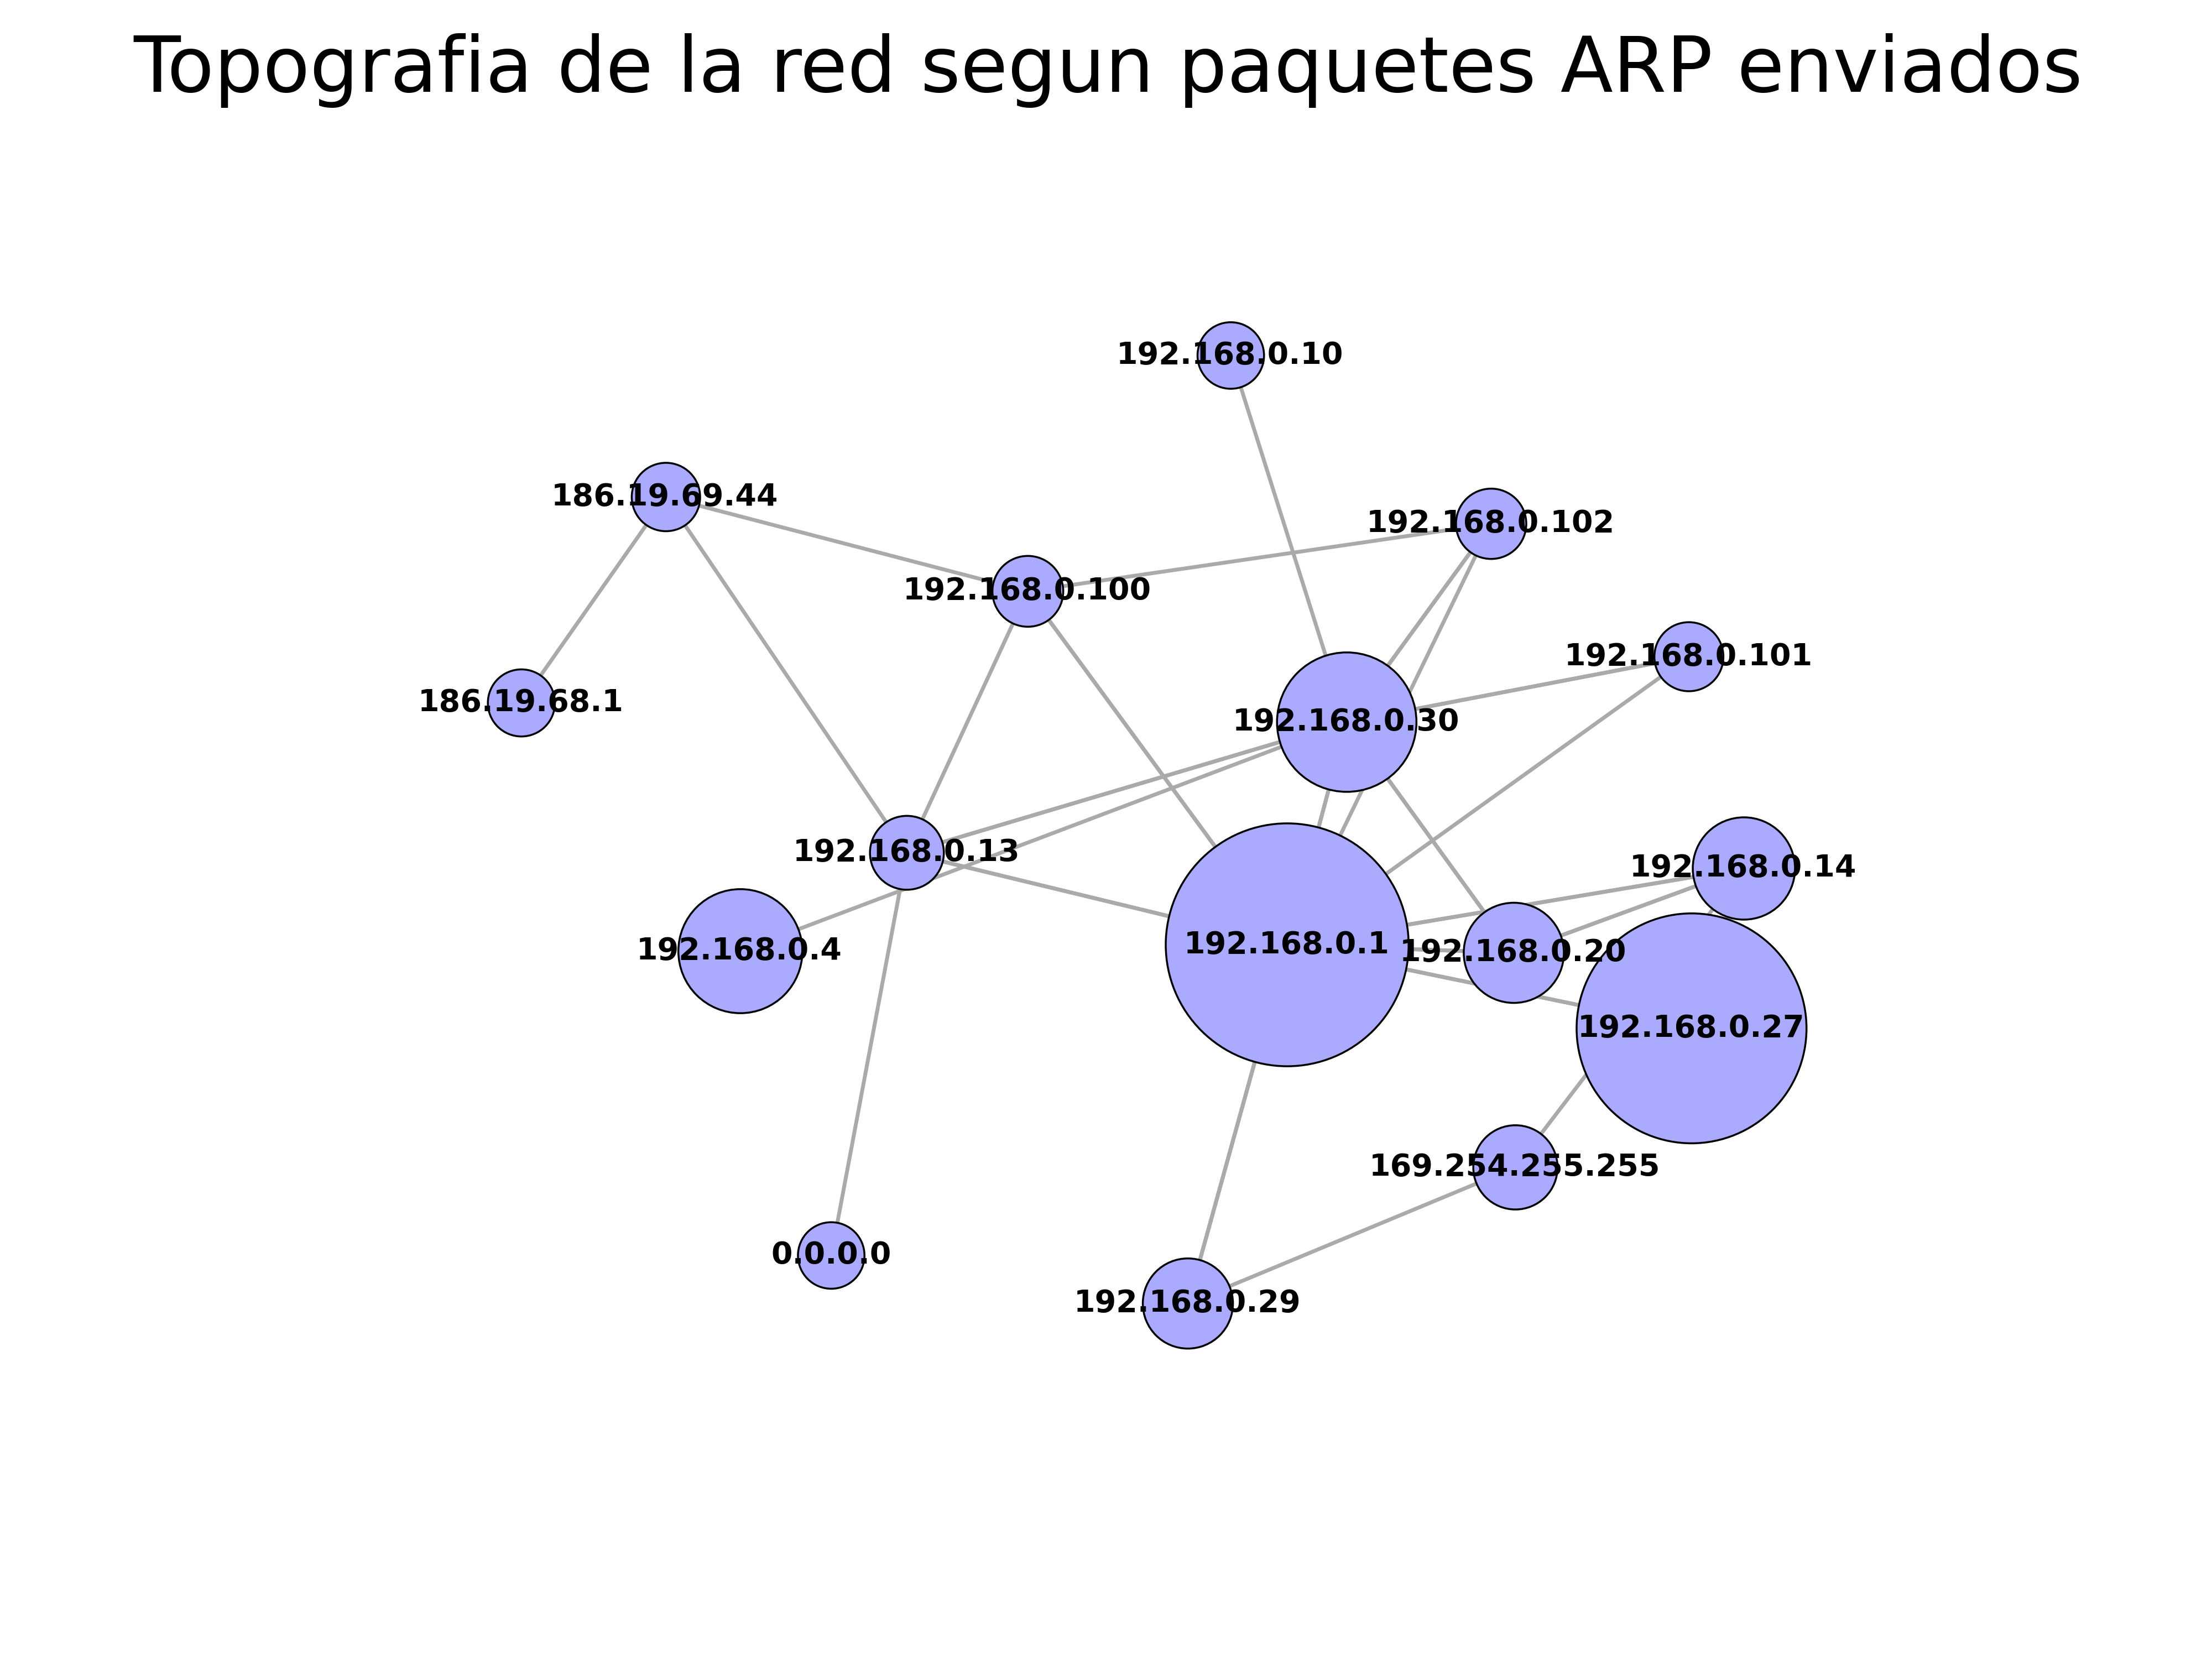
\includegraphics[width=0.7\textwidth]{graficos/red_domestica_network.png}
  \caption{Mi Figura}
  \label{fig:red_domestica_network}
\end{figure}

\FloatBarrier

\subsubsection{Histogramas (de IPs y protocolos)}

\begin{figure}[h!]
  \centering
   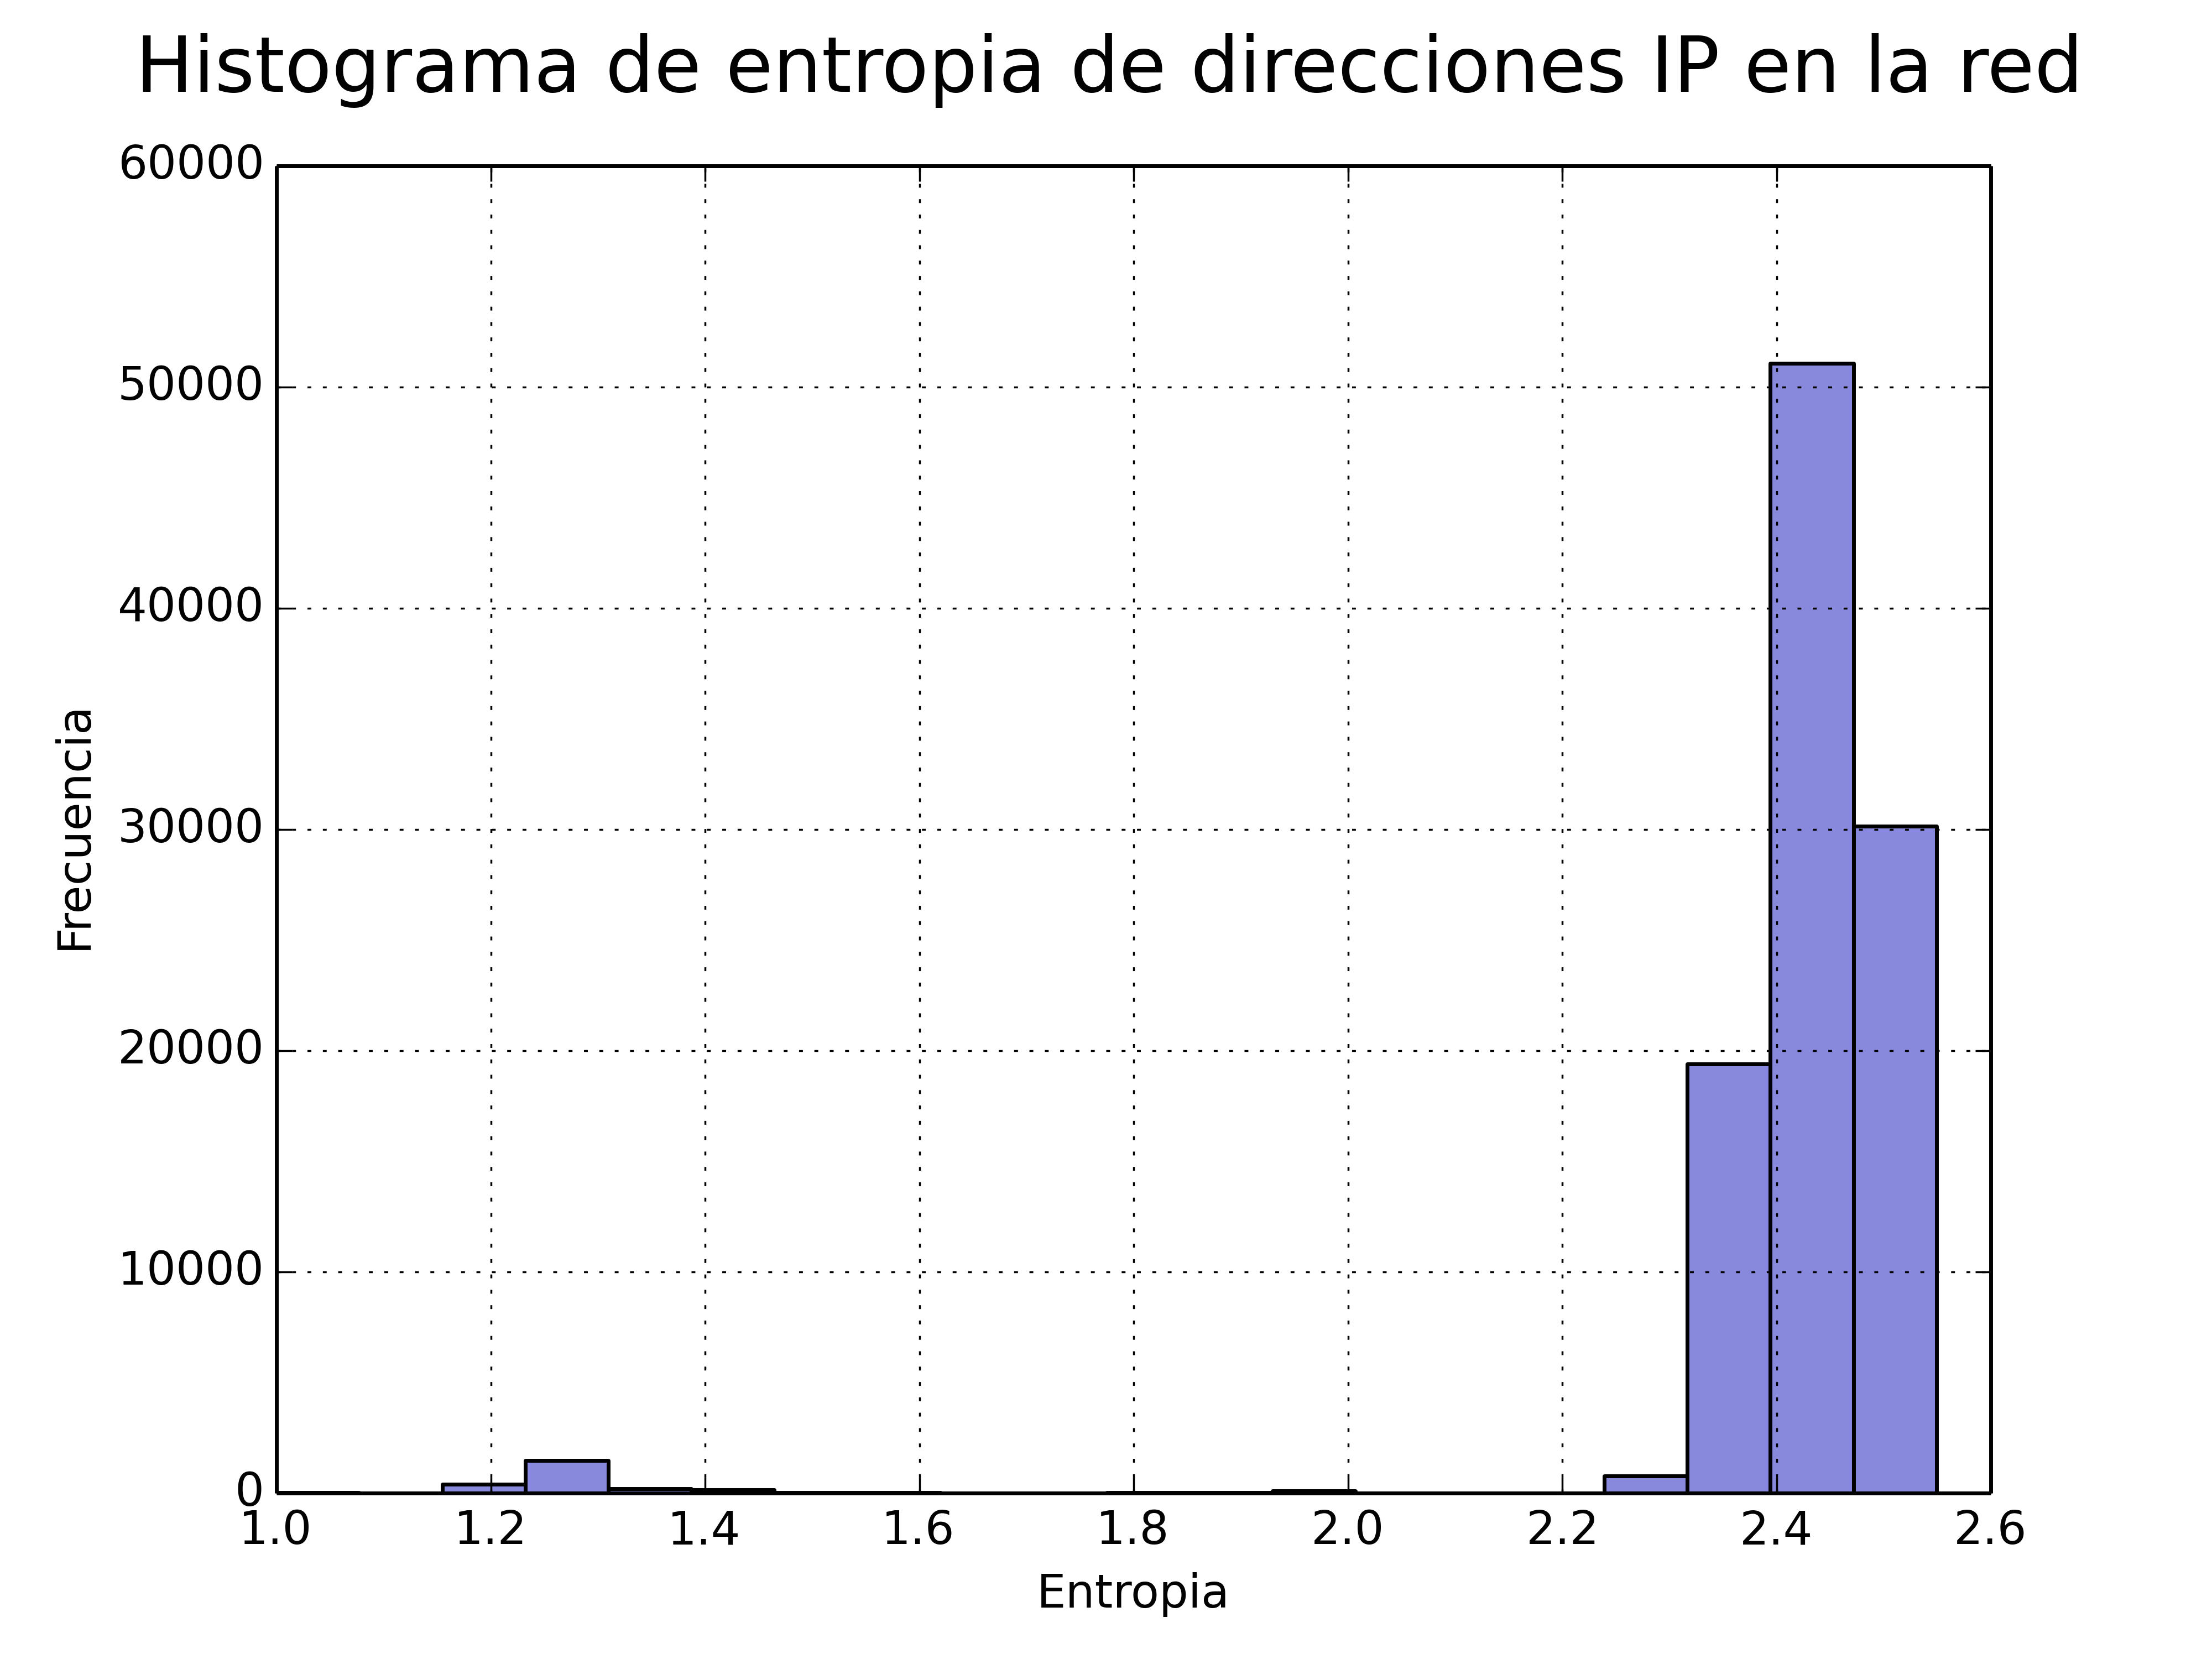
\includegraphics[width=0.7\textwidth]{graficos/red_domestica_hist_arp.png}
  \caption{Mi Figura}
  \label{fig:red_domestica_hist_arp}
\end{figure}

\begin{figure}[h!]
  \centering
   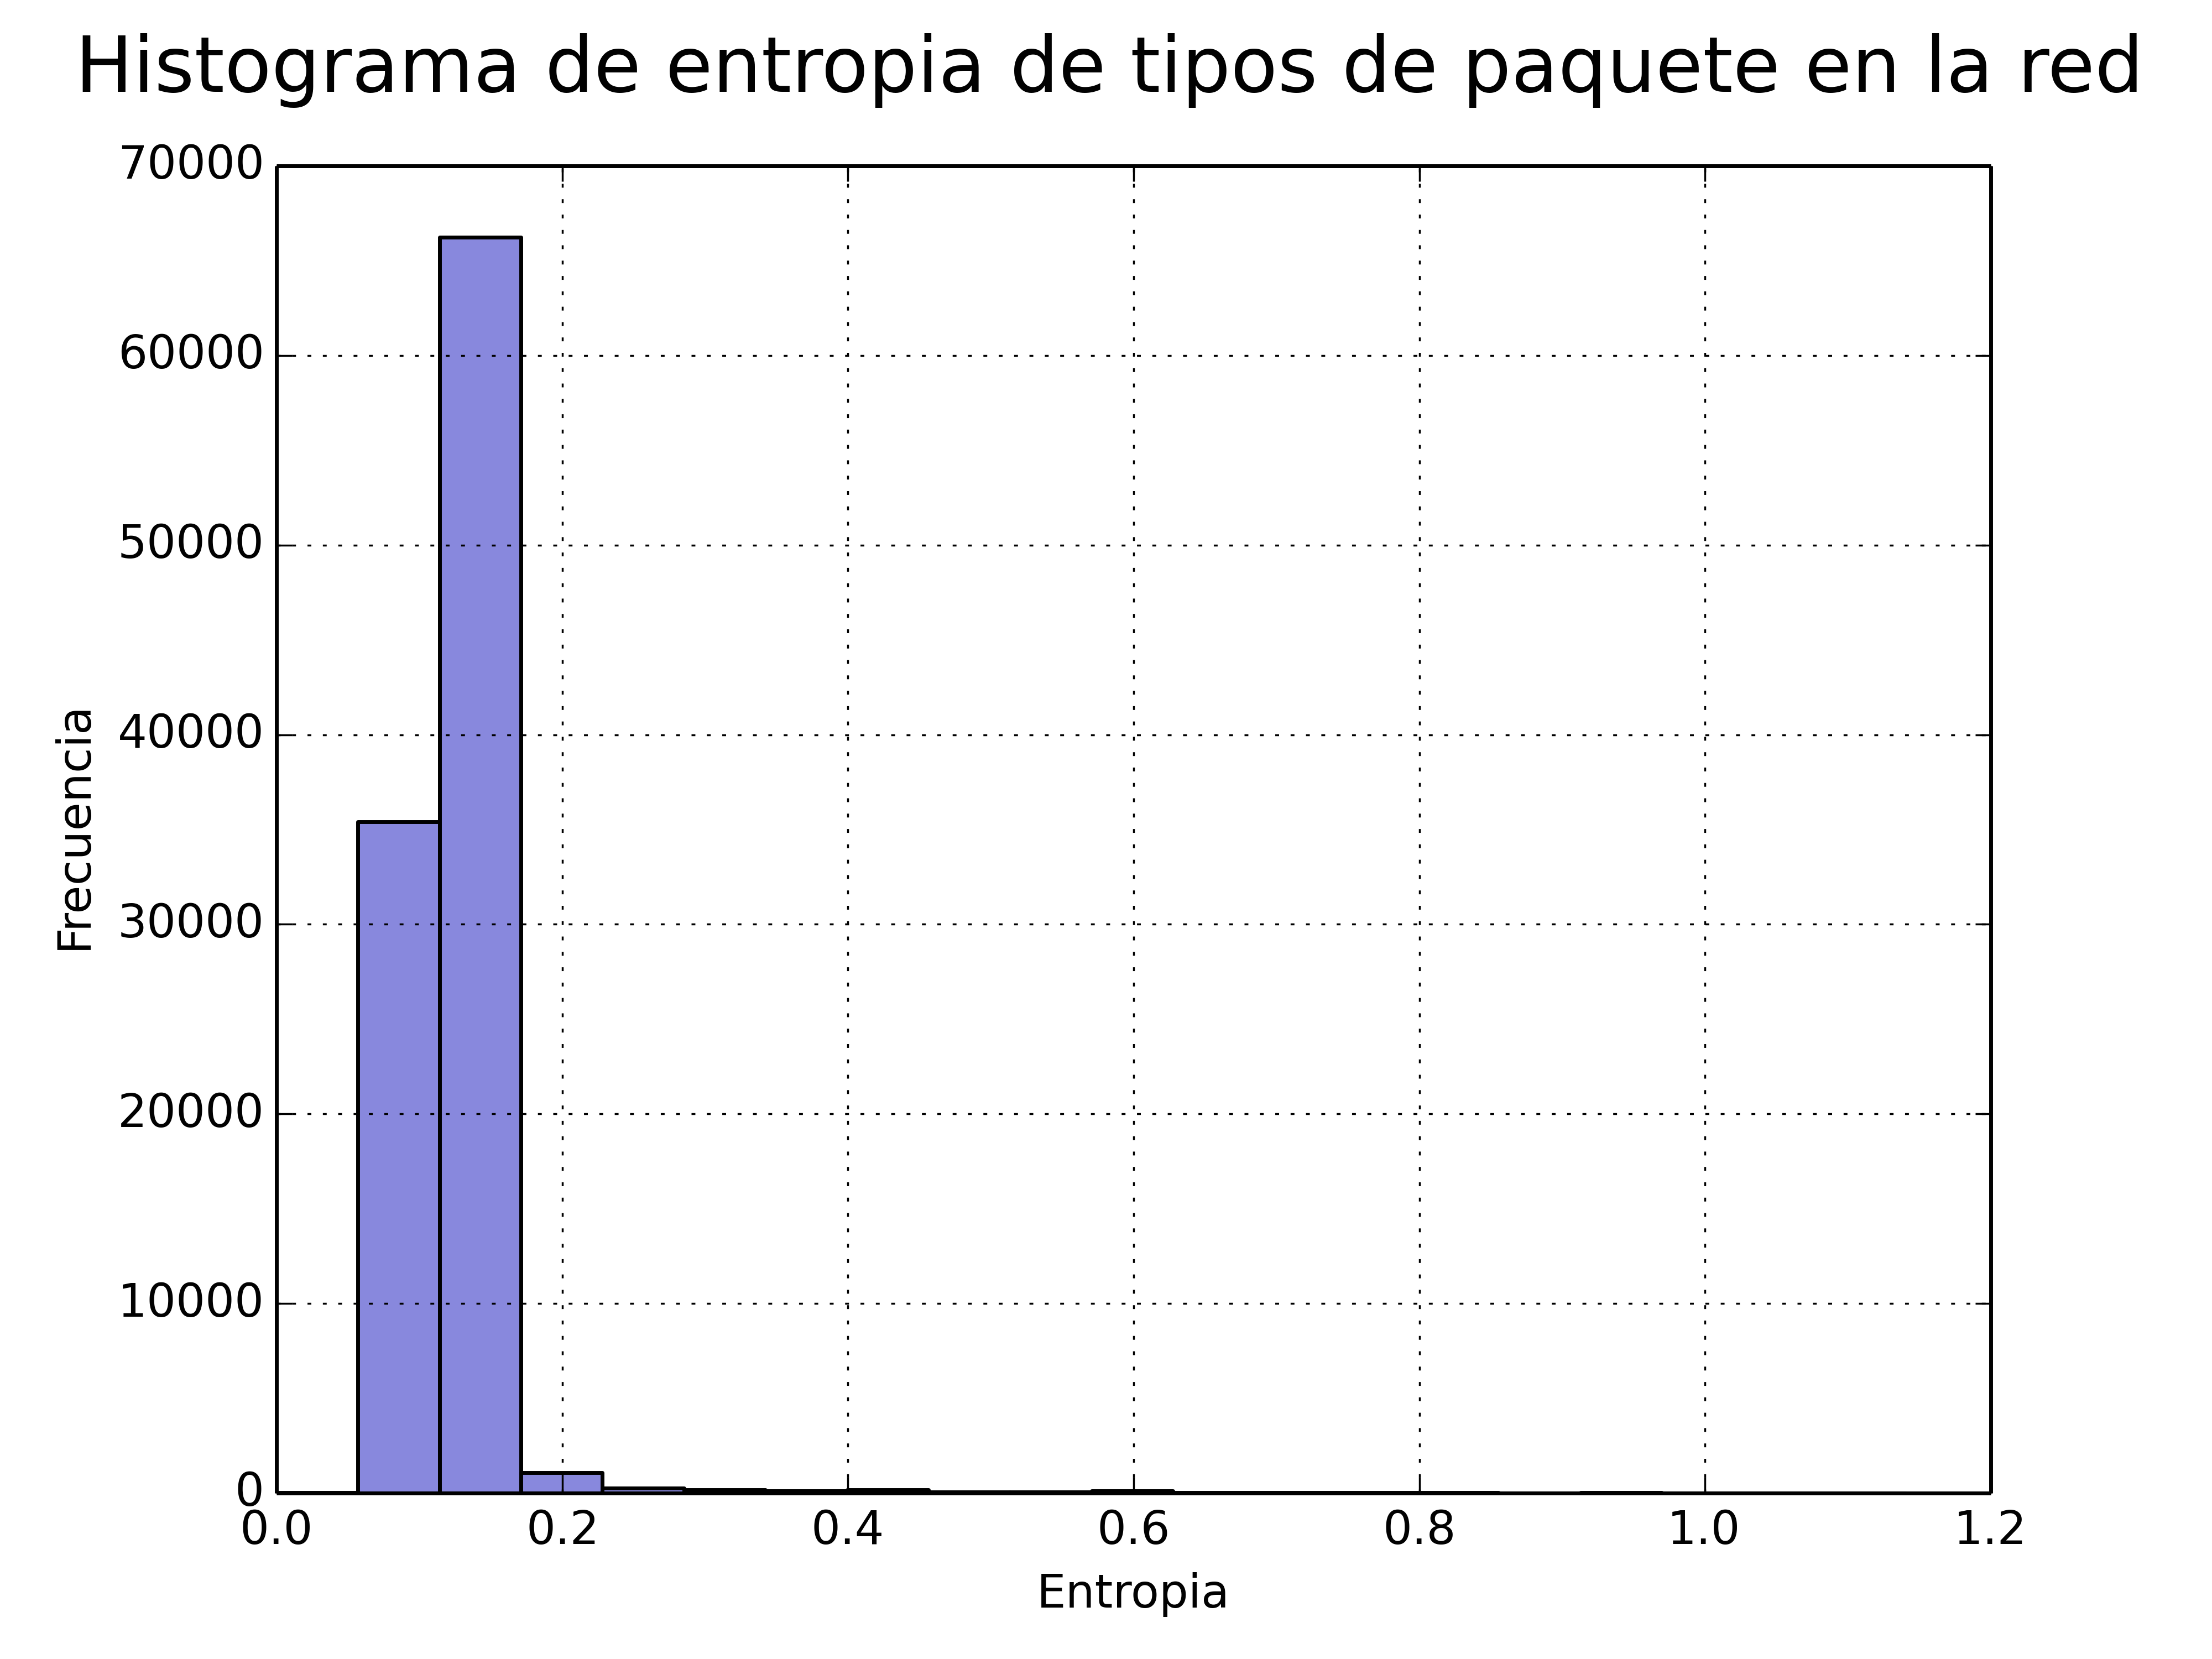
\includegraphics[width=0.7\textwidth]{graficos/red_domestica_hist_type.png}
  \caption{Mi Figura}
  \label{fig:red_domestica_hist_type}
\end{figure}

\FloatBarrier

\subsubsection{Paquetes capturados e información}

Los gráficos de torta, nos permiten ver la relación entre la cantidad de paquetes y la información que proveen cada nodo en la red. 
En los primeros 2 gráficos ~\ref{fig:red_domestica_pie_arp}. ~\ref{fig:red_domestica_pie_arp_information}. se toma como fuente las ips de la red.
Podemos notar que los nodos mencionados anteriormente son los mas frecuentes y por lo tanto los que menos información tienen.

En los siguientes 2 gráficos ~\ref{fig:red_domestica_pie_type}. ~\ref{fig:red_domestica_pie_type_information}. la fuente es la indicada en la cátedra. Vemos que el protocolo que mas se repite es el IP con un porcentaje muy superior al resto y aportando información casi nula. 

\begin{figure}[h!]
  \centering
   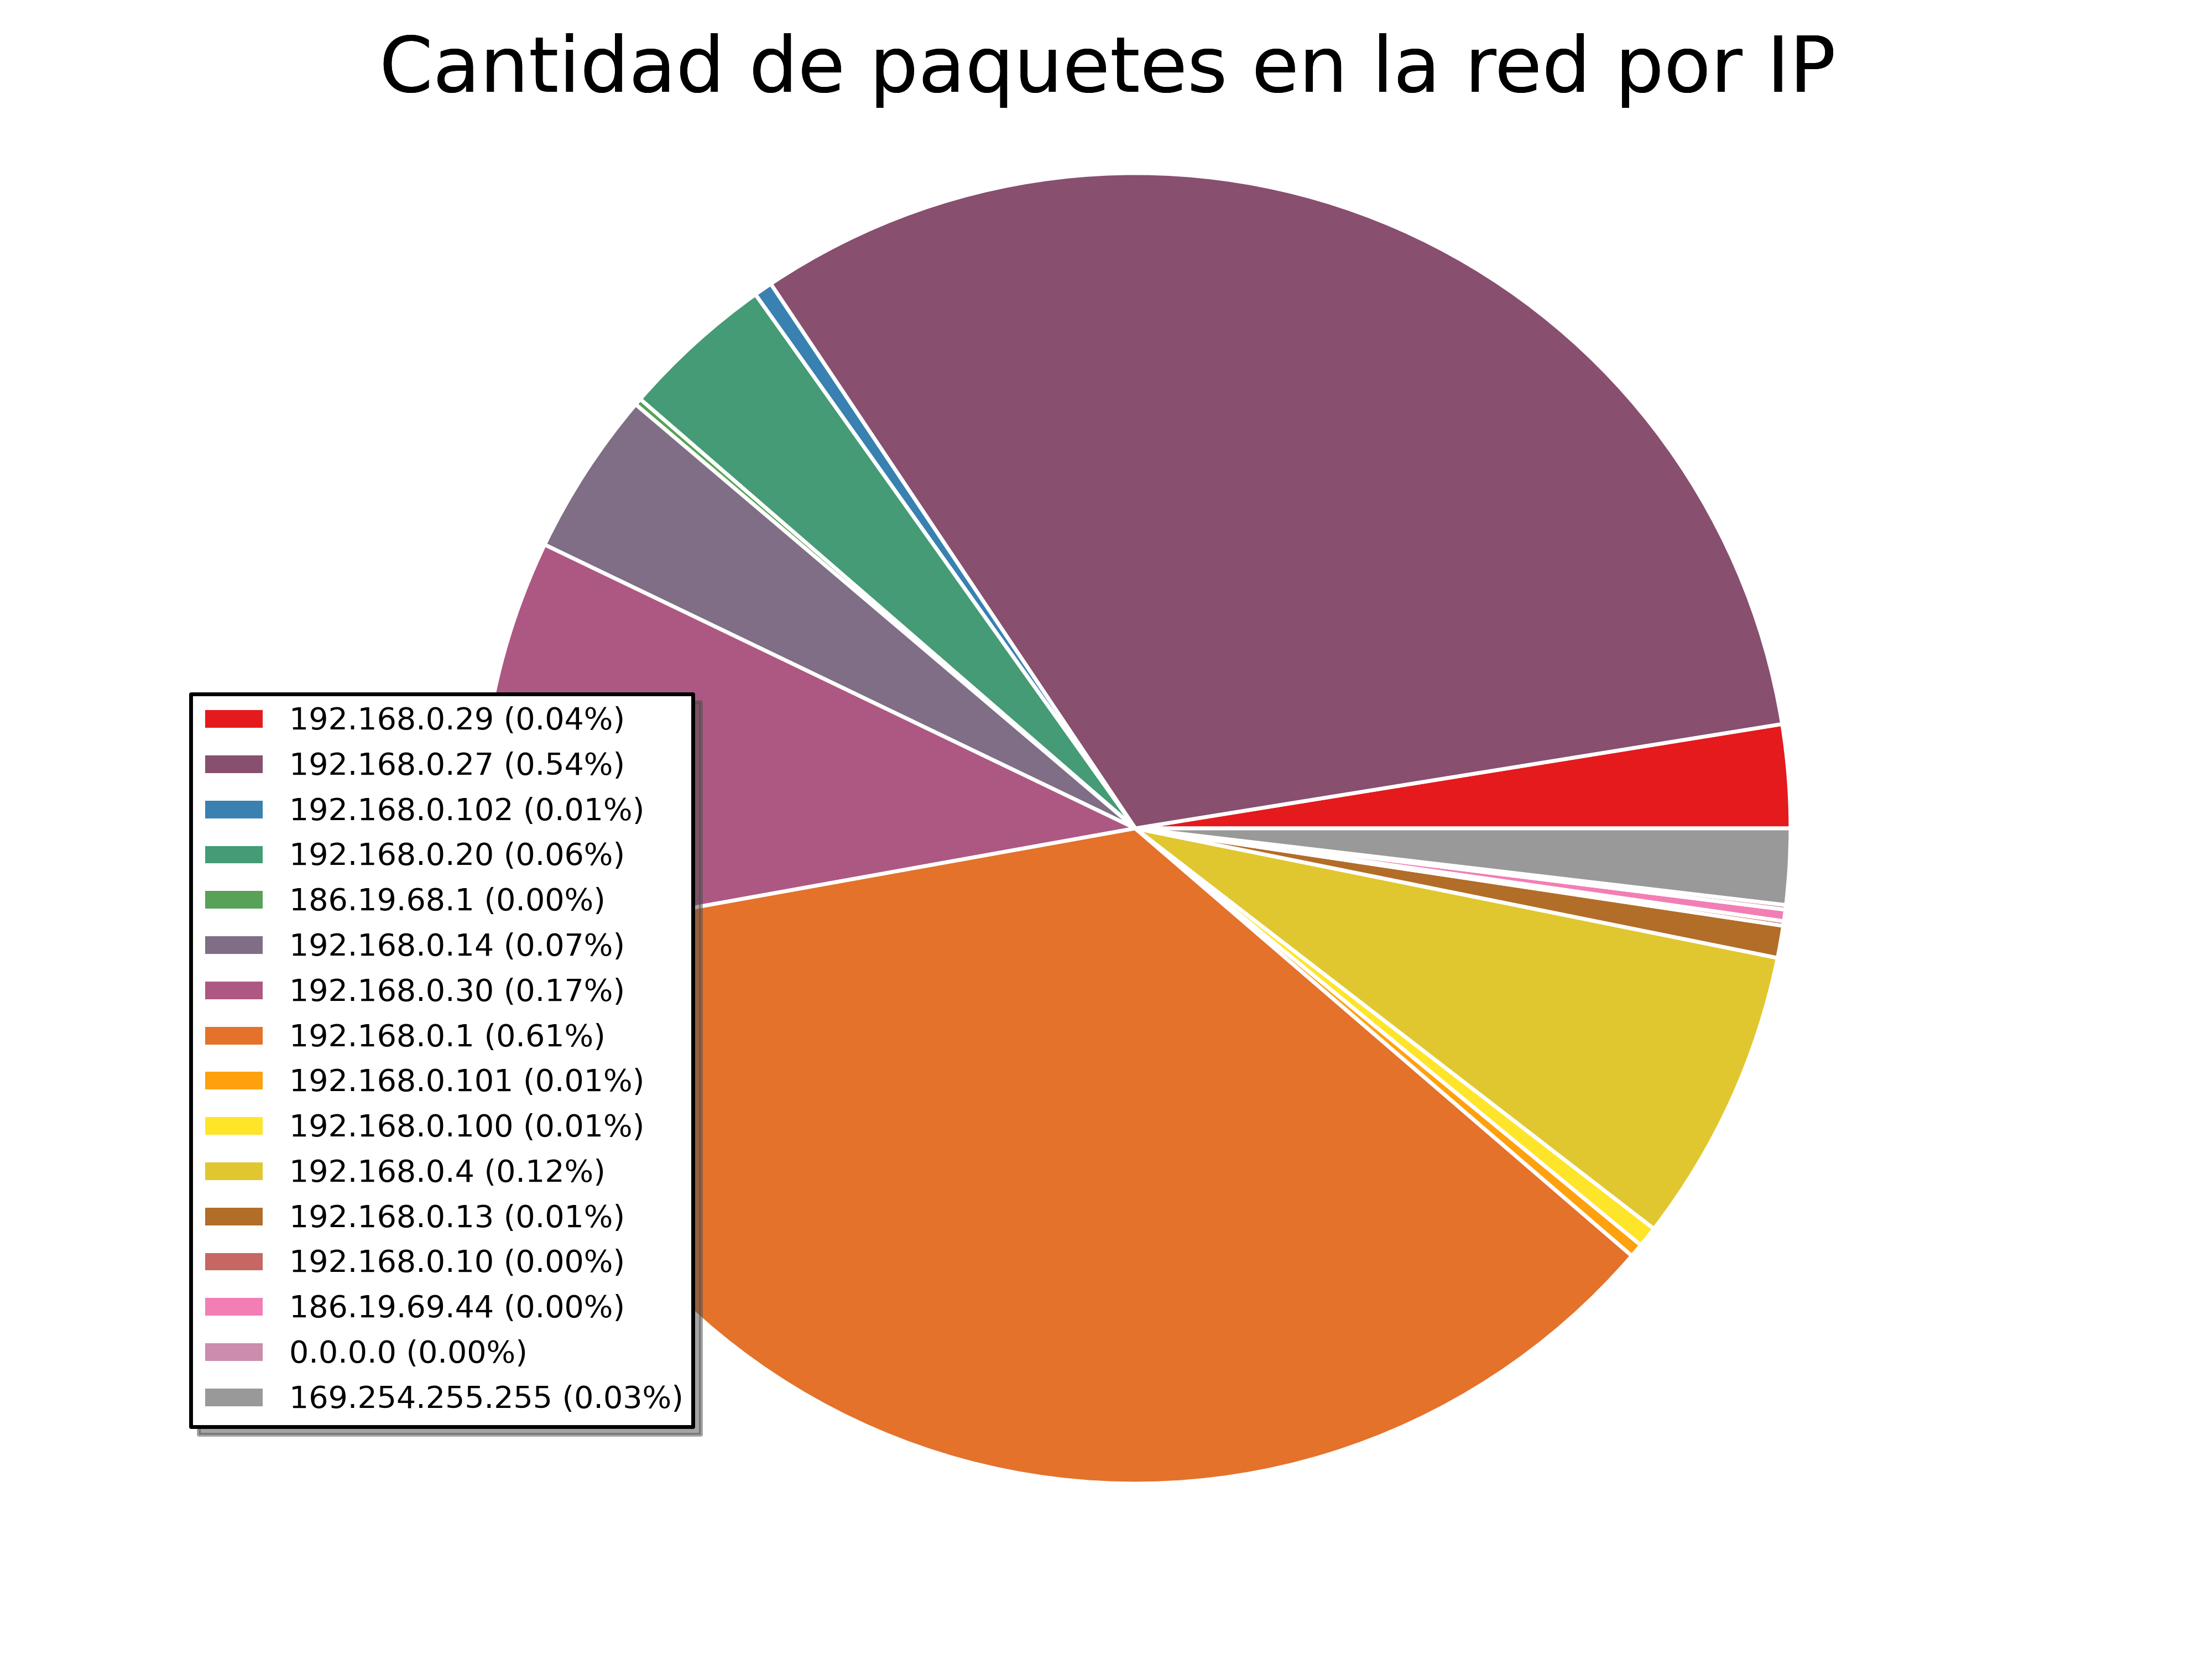
\includegraphics[width=0.7\textwidth]{graficos/red_domestica_pie_arp.png}
  \caption{Mi Figura}
  \label{fig:red_domestica_pie_arp}
\end{figure}

\begin{figure}[h!]
  \centering
   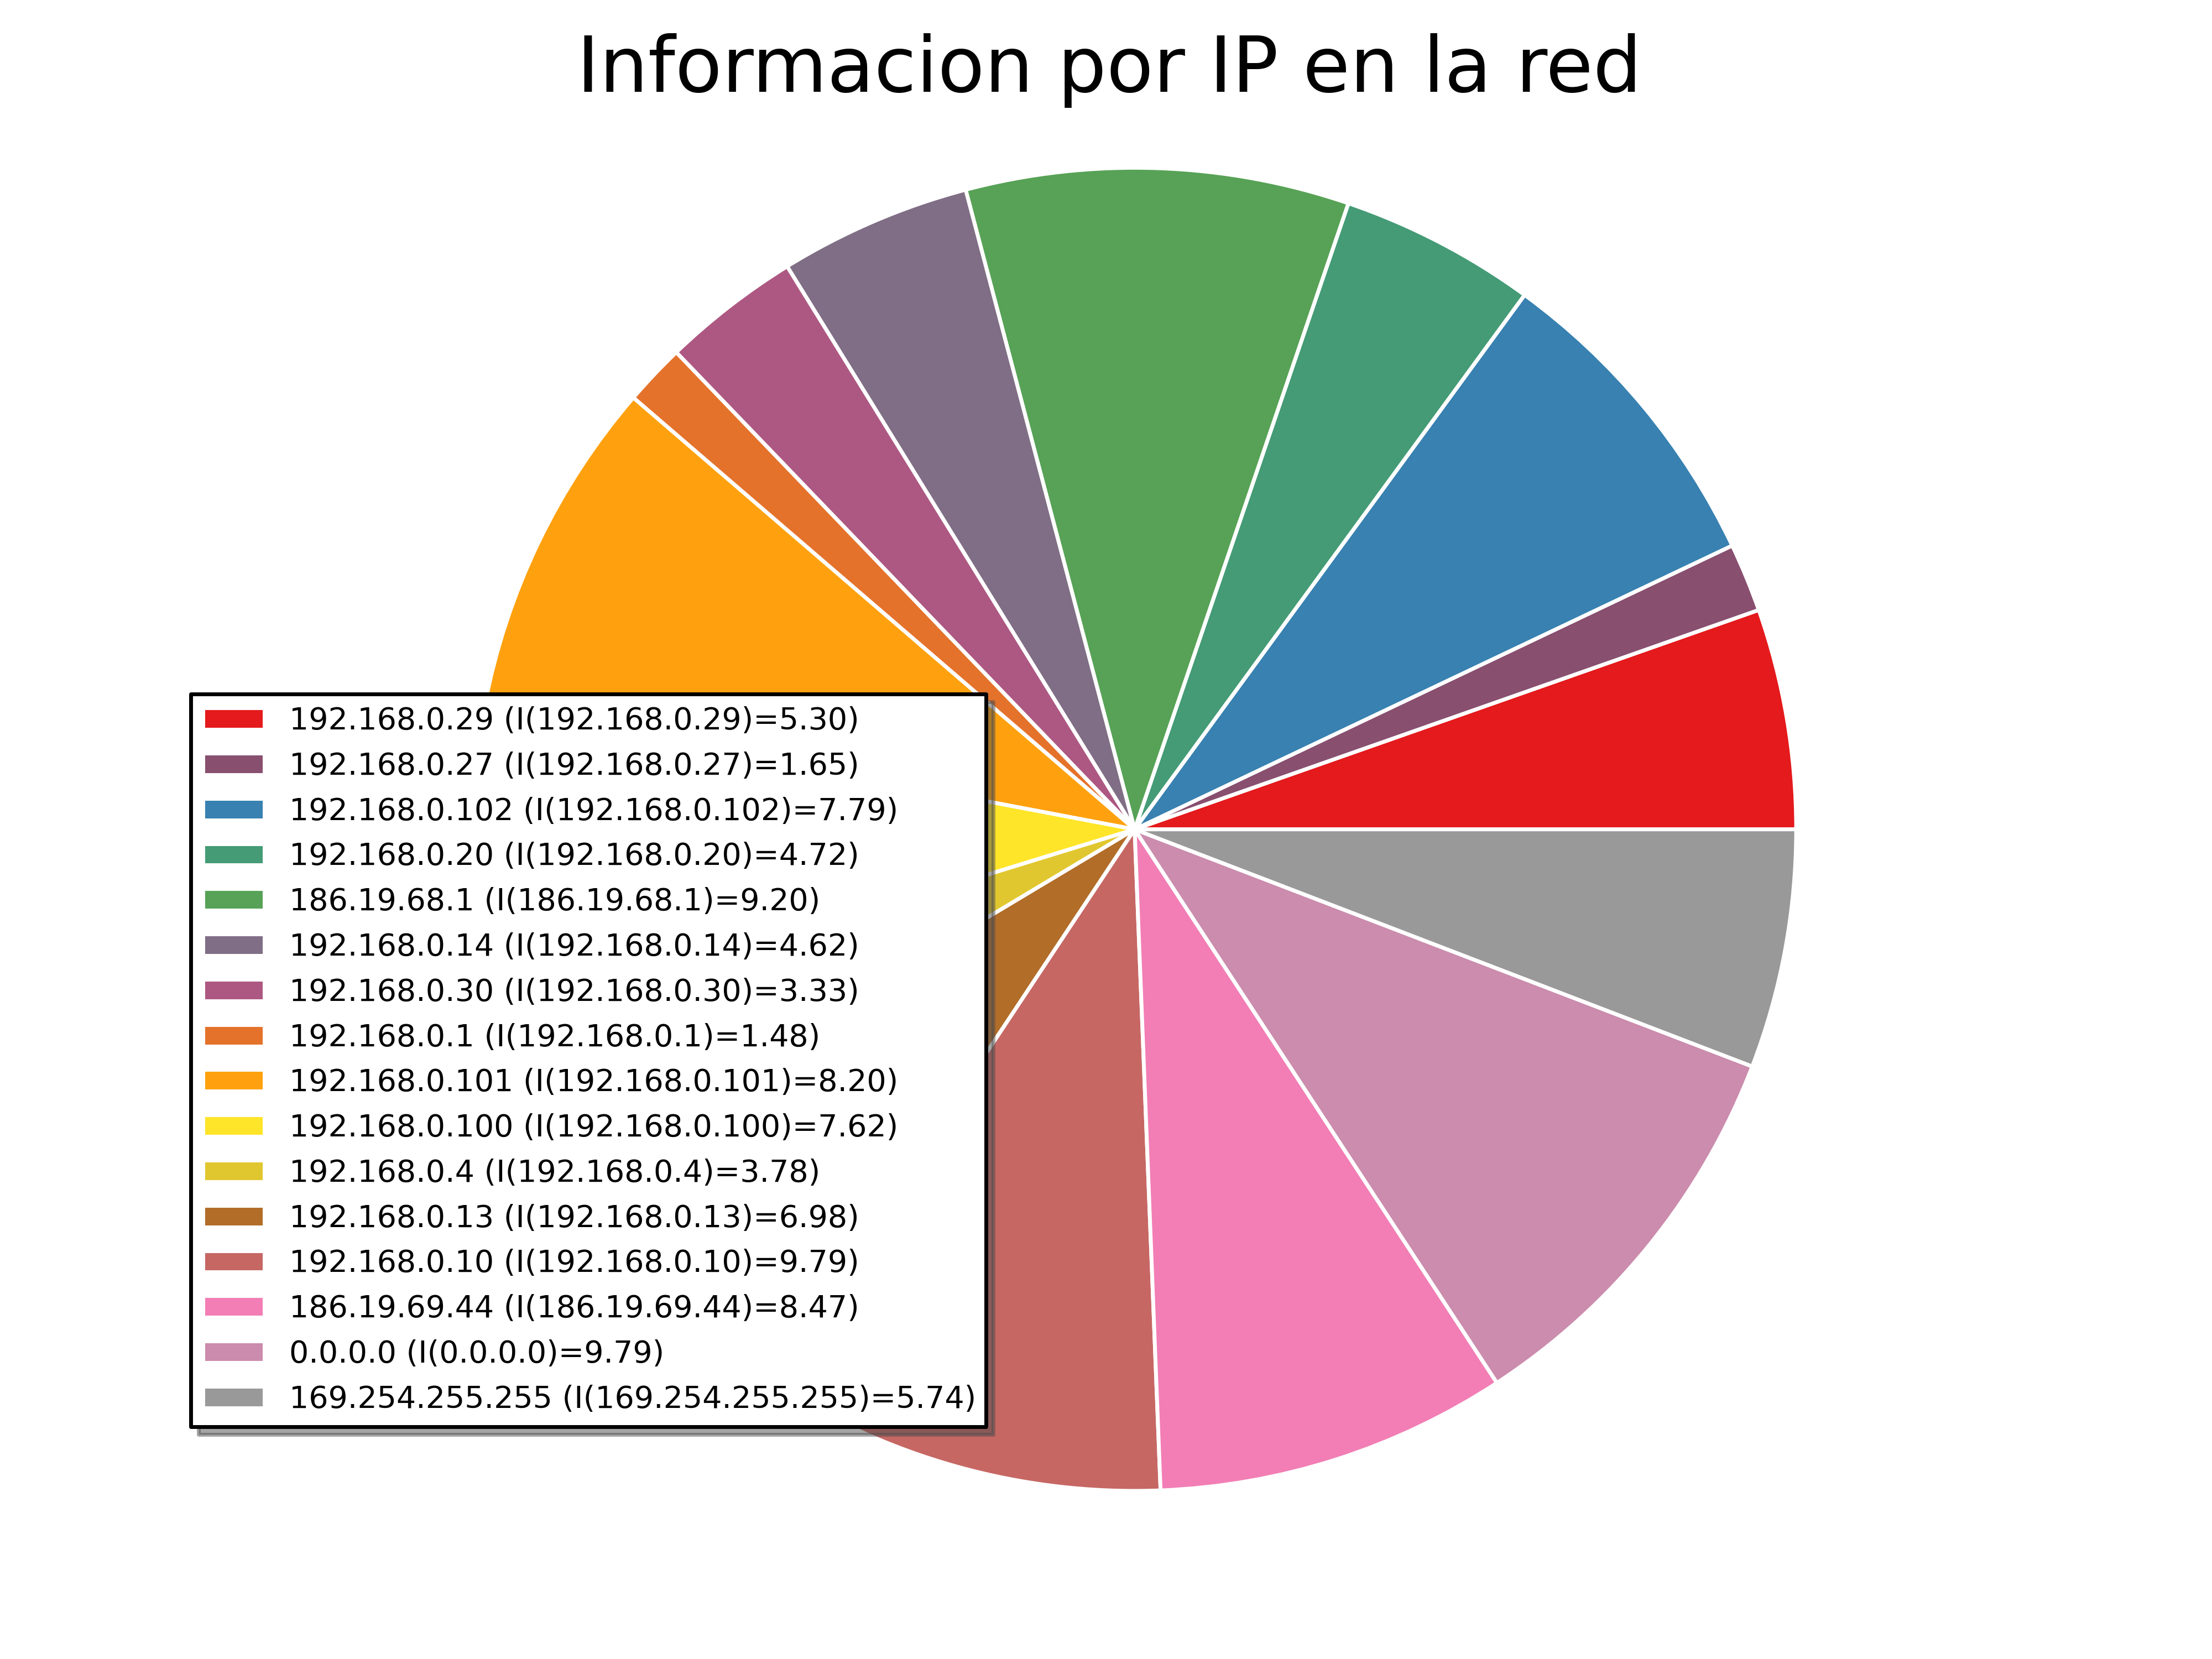
\includegraphics[width=0.7\textwidth]{graficos/red_domestica_pie_arp_information.png}
  \caption{Mi Figura}
  \label{fig:red_domestica_pie_arp_information}
\end{figure}

\begin{figure}[h!]
  \centering
   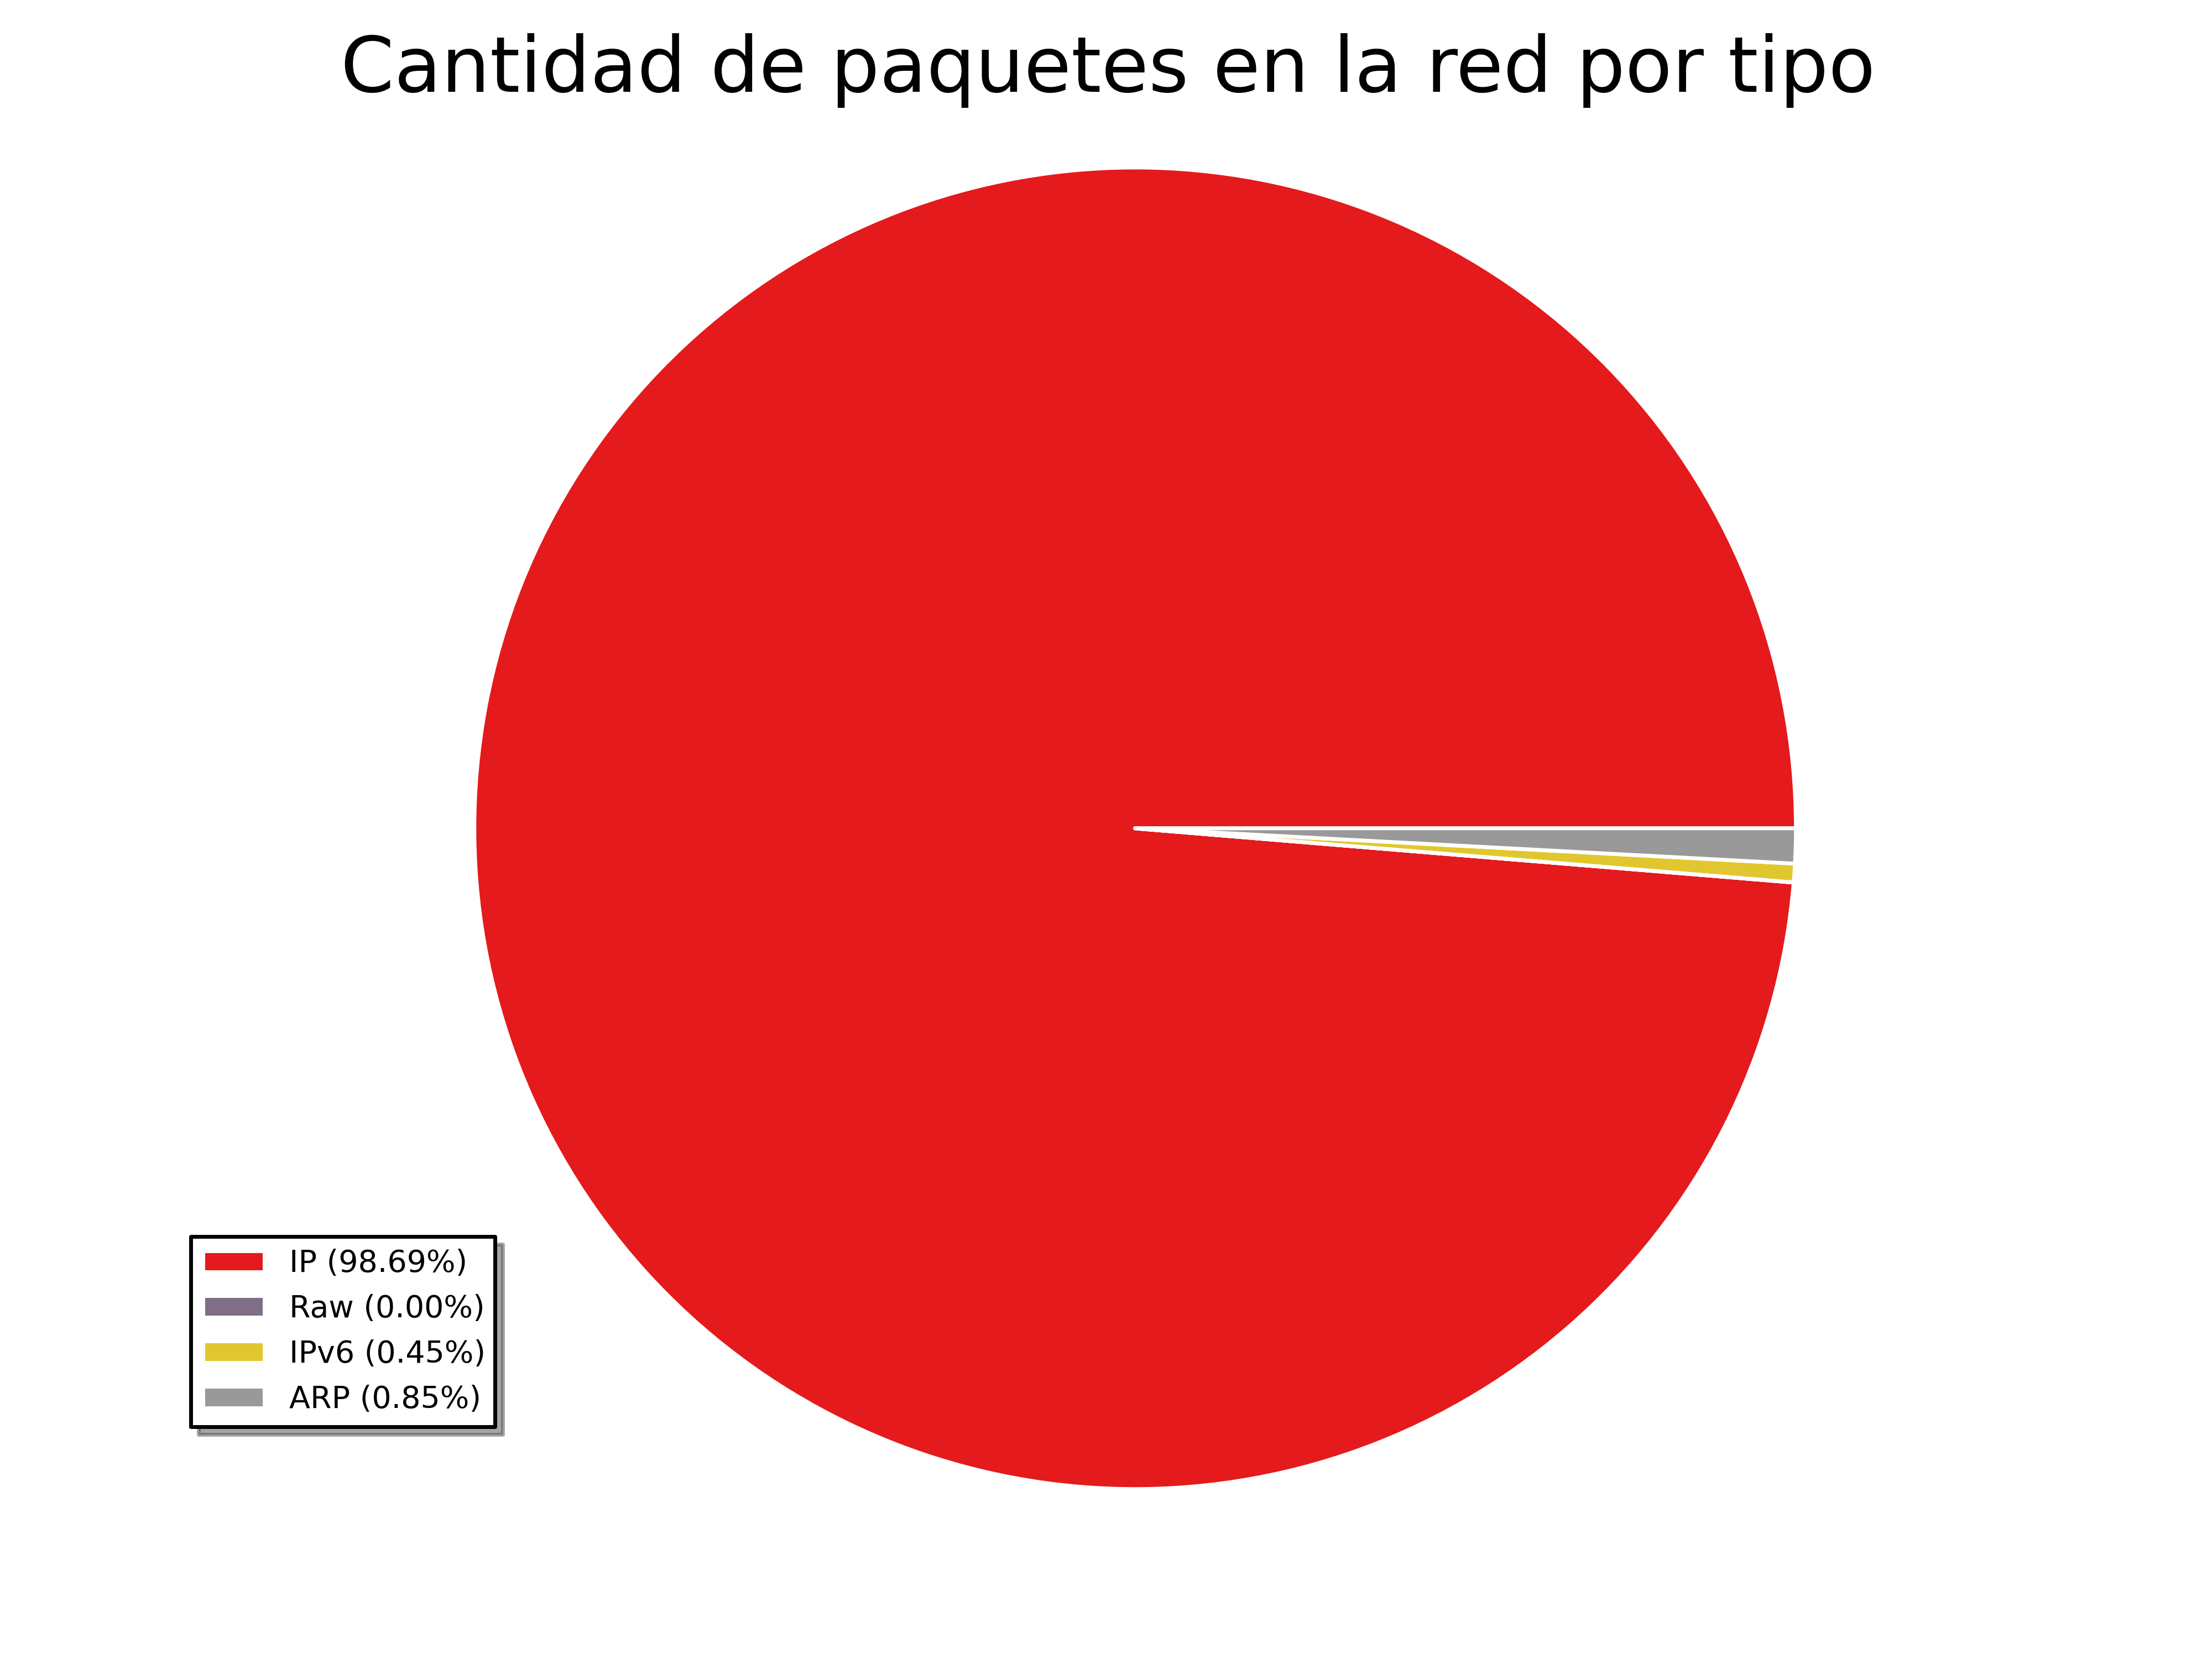
\includegraphics[width=0.7\textwidth]{graficos/red_domestica_pie_type.png}
  \caption{Mi Figura}
  \label{fig:red_domestica_pie_type}
\end{figure}

\begin{figure}[h!]
  \centering
   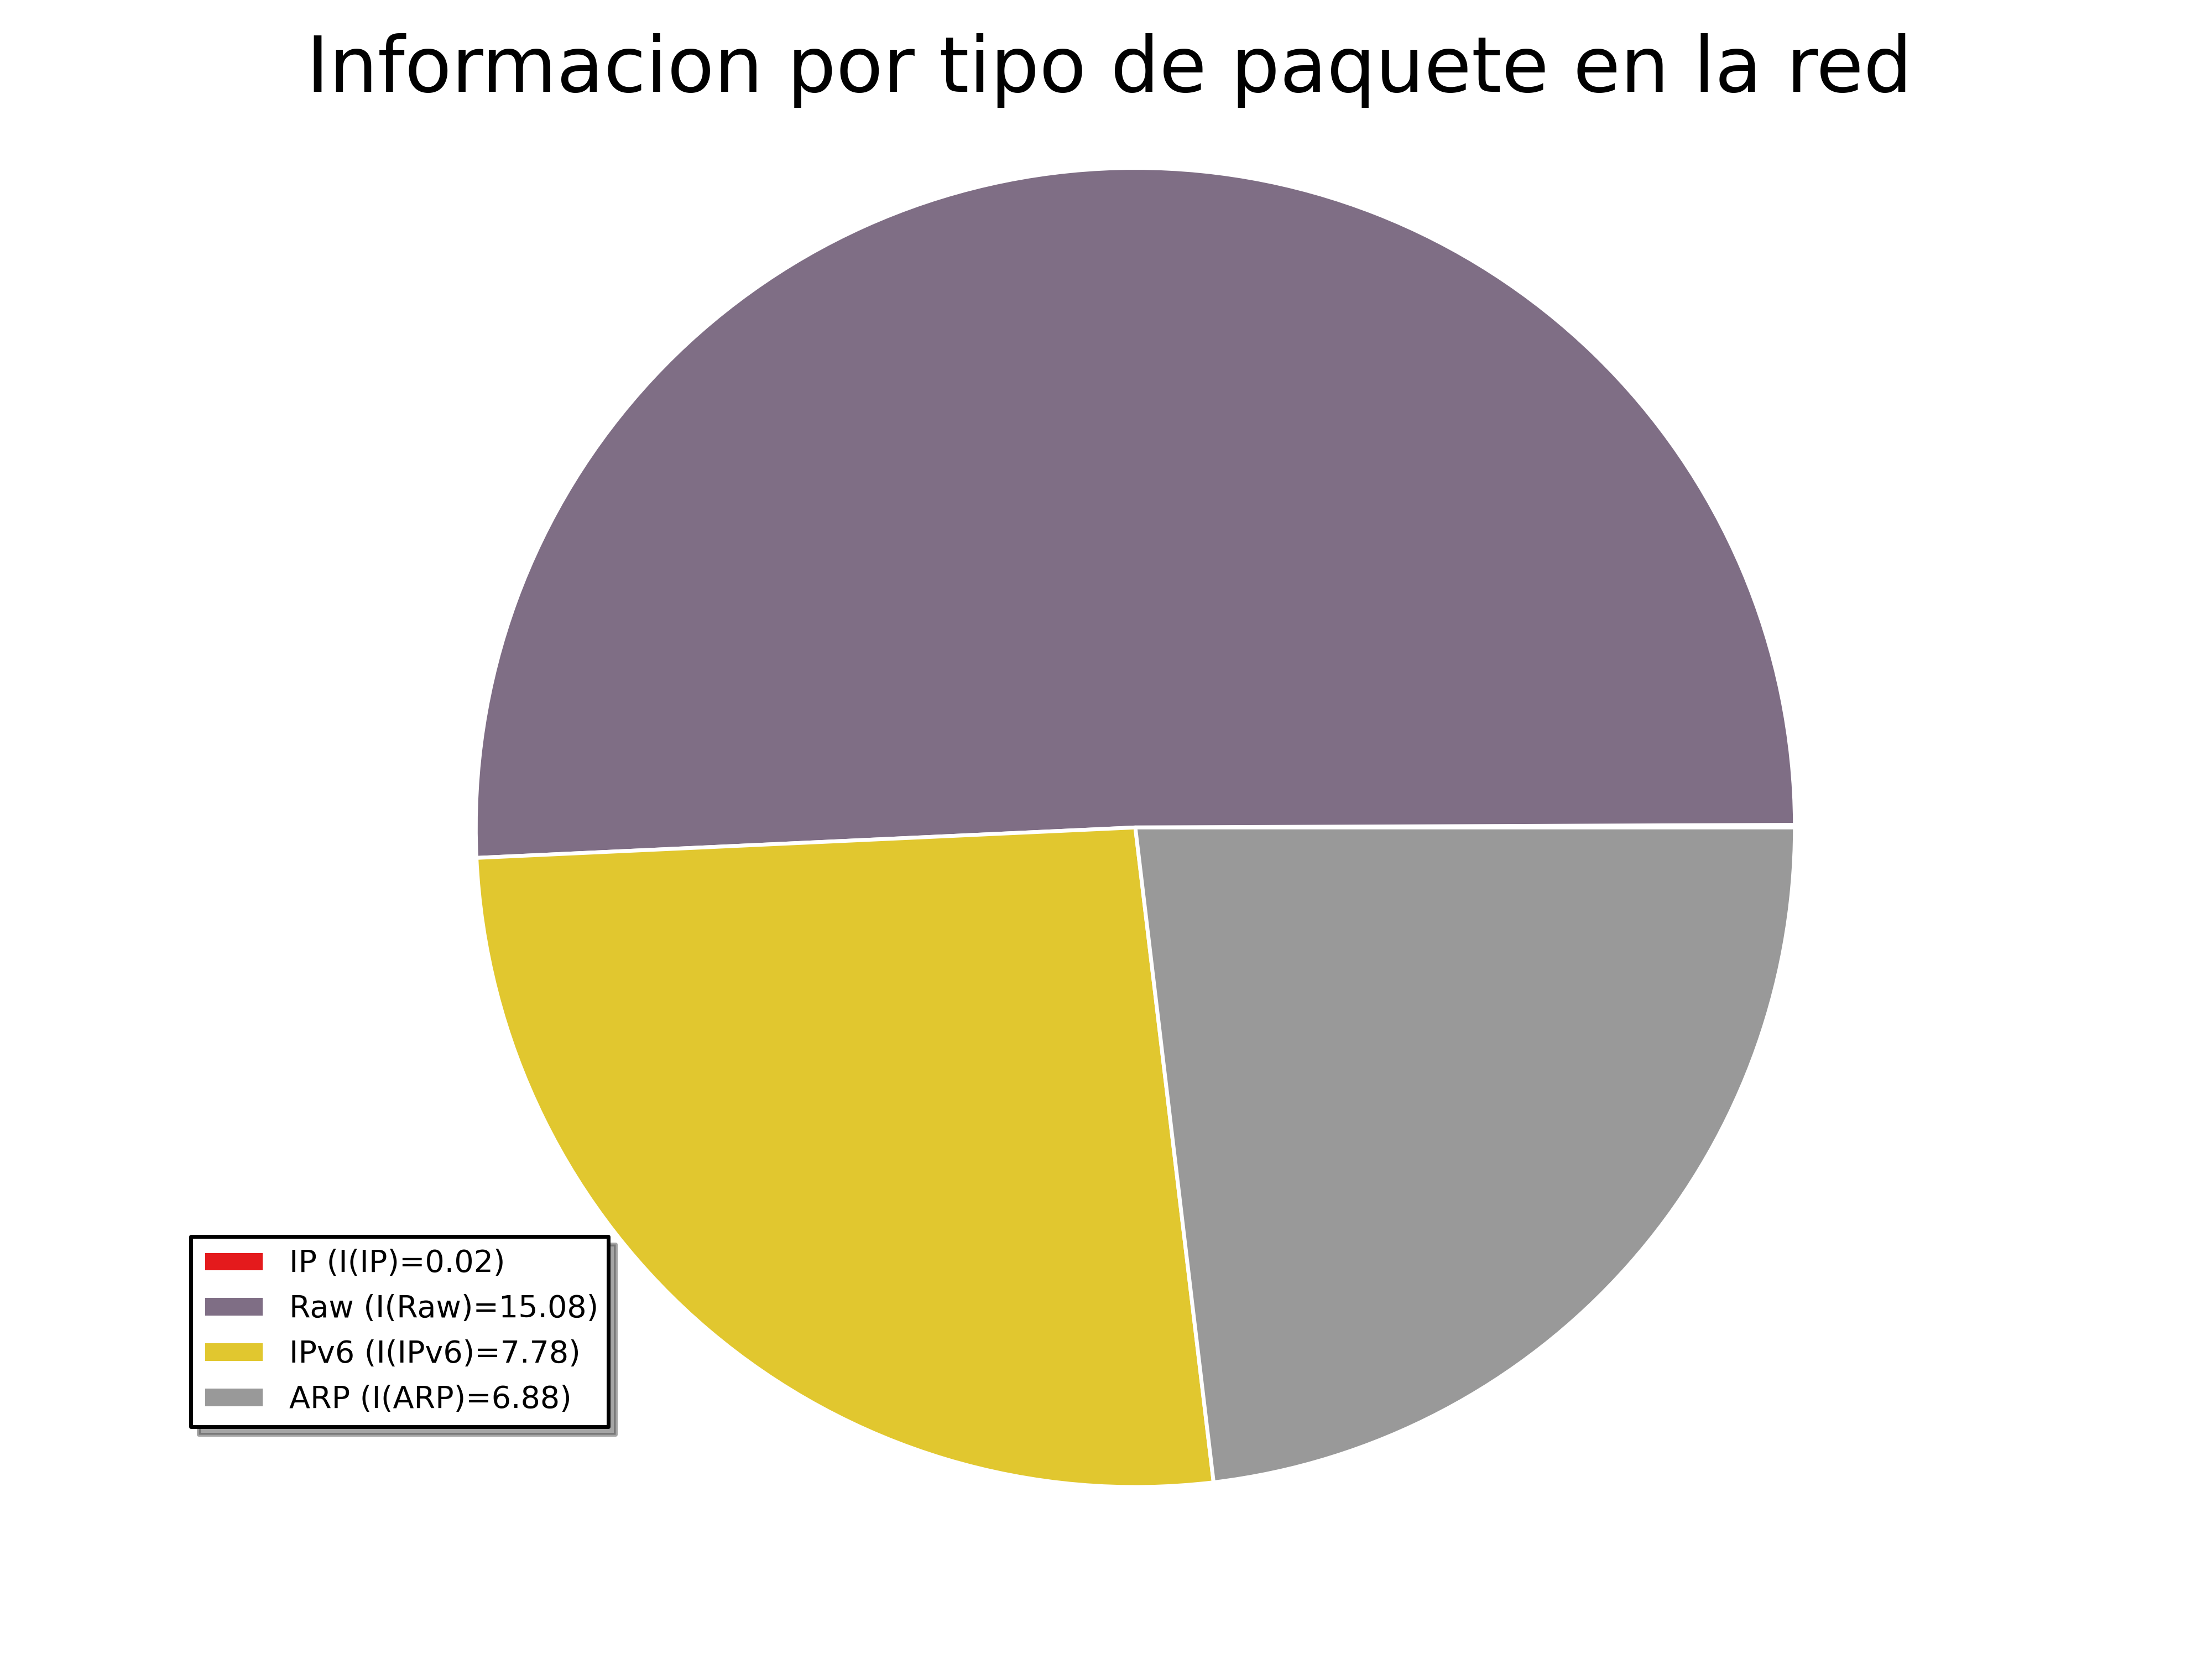
\includegraphics[width=0.7\textwidth]{graficos/red_domestica_pie_type_information.png}
  \caption{Mi Figura}
  \label{fig:red_domestica_pie_type_information}
\end{figure}
\newpage
\section{Conclusiones}
En estos experimentos pudimos apreciar una aplicación concreta de la teoría de la información que nos permitió modelar y analizar diferentes fuentes de información.
\\\\
En la primera parte del trabajo práctico, al buscar protocolos distinguidos se descubrió que, en general, el protocolo más frecuente es el IPv4, lo cual es razonable. Además se notó que en algunas redes el protocolo IPv6, también, es bastante frecuente y que el protocolo ARP siempre se encontró presente en ellas. Esto último es previsible, por el funcionamiento de las redes IP en LAN.
\\\\
En el análisis de protocolos pudimos encontrar muchas similitudes entre las distintas redes. En general la entropía de esta fuente presentó un valor bajo y además el protocolo IPv4, que es el que mayor tráfico presenta, aportó valores de información inferiores. Esto demuestra una fuente predecible en la que se espera que la mayoría de los paquetes pertenezcan al protocolo IPv4.
\\\\
En la segunda parte del trabajo se investigó la existencia de nodos distinguidos (o símbolos distinguidos en el contexto de la fuente $S_1$).
\\\\
Se pudo observar que en las redes analizadas el router fue uno de los nodos distinguidos.
\\\\
También se observó que para las fuentes que modelan los diferentes nodos de la red, el valor de la entropía fue más elevado que la entropía de las fuentes que modelan los tipos de protocolos. Esto nos parece razonable debido a la impredecibilidad de la incidencia de los nodos en la red en comparación con la de los diferentes tipos de protocolos.


\newpage



%\newpage
%\begin{thebibliography}{9}
 %\end{thebibliography}


\end{document}

